\documentclass{webofc}
\usepackage[varg]{txfonts}
\usepackage{natbib}

\usepackage{xcolor}

\usepackage[justification=centering]{caption}

\begin{document}

\title{BigPanDA: PanDA Workload Management System and its Applications beyond ATLAS}

%\author{
%  \firstname{Andre} \lastname{Merzky}\inst{2} \and
%  \firstname{Pavlo} \lastname{Svirin}\inst{1} \and
%  \firstname{Matteo} \lastname{Turilli}\inst{2}
%}


\author{
%P. Svirin1, K. De2, A. Forti3, A. Klimentov1, R. Larsen1, P. Love4, T. Maeno1, R. Mashinistov1, S. Mukherjee1, A. Nomerotski1, D. Oleynik2, S. Panitkin1, H. Park1,5, E. Sheldon1, A. Slosar1, J. Wells6 and T. Wenaus1
\firstname{Pavlo} \lastname{Svirin}\inst{1} \and
\firstname{Kaushik} \lastname{De}\inst{2} \and
\firstname{Alessandra} \lastname{Forti}\inst{3} \and
\firstname{Alexei} \lastname{Klimentov}\inst{1} \and
\firstname{Rasmus} \lastname{Larsen}\inst{1} \and
\firstname{Peter} \lastname{Love}\inst{4} \and
\firstname{Tadashi} \lastname{Maeno}\inst{1} \and
\firstname{Ruslan} \lastname{Mashinistov}\inst{1} \and
\firstname{Swagato} \lastname{Mukherjee}\inst{1} \and
\firstname{Andrei} \lastname{Nomerotski}\inst{1} \and
\firstname{Danila} \lastname{Oleynik}\inst{2} \and
\firstname{Sergey} \lastname{Panitkin}\inst{1} \and
\firstname{Heyun} \lastname{Park}\inst{1,5} \and
\firstname{Erin} \lastname{Sheldon}\inst{1} \and
\firstname{Anze} \lastname{Slosar}\inst{1} \and
\firstname{Jack} \lastname{Wells }\inst{6} \and
\firstname{Torre} \lastname{Wenaus}\inst{1}
%  \firstname{Andre} \lastname{Merzky}\inst{2} \and
%  \firstname{Pavlo} \lastname{Svirin}\inst{1} \and
%  \firstname{Matteo} \lastname{Turilli}\inst{2}
}

\institute{
Brookhaven National Laboratory (BNL), Upton, NY USA \and 
University of Texas at Arlington (UTA), Arlington, TX USA \and 
School of Physics and Astronomy, University of Manchester, Manchester, United Kingdom		 	 	  \and 
Physics Department, Lancaster University, Lancaster, United Kingdom \and 
Stony Brook University (SBU), Stony Brook, NY USA  \and 
Oak Ridge National Laboratory (ORNL), Oak Ridge, TN USA 
}

\abstract{Modern experiments collect peta-scale volumes of data and utilize vast, geographically distributed computing infrastructure that serves thousands of scientists around the world. Requirements for rapid, near real-time data processing, fast analysis cycles and need to run massive detector simulations to support data analysis pose special premium on efficient use of available computational resources.

A sophisticated Workload Management System (WMS)  is needed to coordinate the distribution and processing of data and jobs in such environment. The ATLAS experiment at CERN uses PanDA (Production and Data Analysis) Workload Management System for managing the workflow for all data processing on over 150 data centers. While PanDA currently uses more than 250,000 cores with a peak performance of 0.3 petaFLOPS, it runs around 2 million jobs per day on hundreds of Grid sites and serving thousands of ATLAS users. In 2017 about 1.5 exabytes of data were processed with PanDA.

In 2012 BigPanDA project project was started with aim to introduce new types of computing resources into ATLAS computing infrastructure, but also to offering PanDA features to different data-intensive applications for projects and experiments outside of ATLAS and High-Energy and Nuclear Physics. In this article we will present accomplishments and discuss possible directions for future work.}

\maketitle

% ---------------------------------------------------------------------------
\section{Introduction}
\label{intro} 

% =============

Production and Distributed Analysis Workload Management System (PanDA WMS) ~\cite{PanDA} is the system initially developed for ATLAS experiment~\cite{ATLAS_Collaboration_2008} and was designed as high-level intellectual layer on WLCG~\cite{doi:10.1146/annurev-nucl-102010-130059} grid-infrastructure. 
%WLCG built on the gLite middleware~\cite{gLite} and released in 2005 already provided the wide range of the services which can be thematically grouped into 5 service groups: Access Services, Security Services, Information and Monitoring Services, Data Services and Job Management Services (Figure~\ref{fig:panda-arch}). 
WLCG built on the gLite middleware~\cite{gLite} and released in 2005 already provided the wide range of services. (Figure~\ref{fig:panda-arch}). 

At the same time parallely developed PanDA system allowed the efficient use of gLite infrastructure and provided a multiple benefits. Most significant features provided by PanDA are the following: 

\begin{itemize}
	\item The implementation of the late-binding principle for the job payload with CPU slots using the Pilots component. Now the standard Grid-job became the carrier of the Pilot-job which in it’s order became responsible of the handling the Payload. 
	\item Brokerage of the jobs in PanDA implemented in highly sophisticated way taking into account many factors of the real ATLAS workflow and workload and integrating multiple components of the computing model. 
	\item Monitoring of the PanDA system is also developed according to the daily necessities of the real users. Being the core component of the ATLAS production system PanDA confidently copes the needs of the experiment since the commissioning. 
\end{itemize}

\begin{figure}
	\centering
	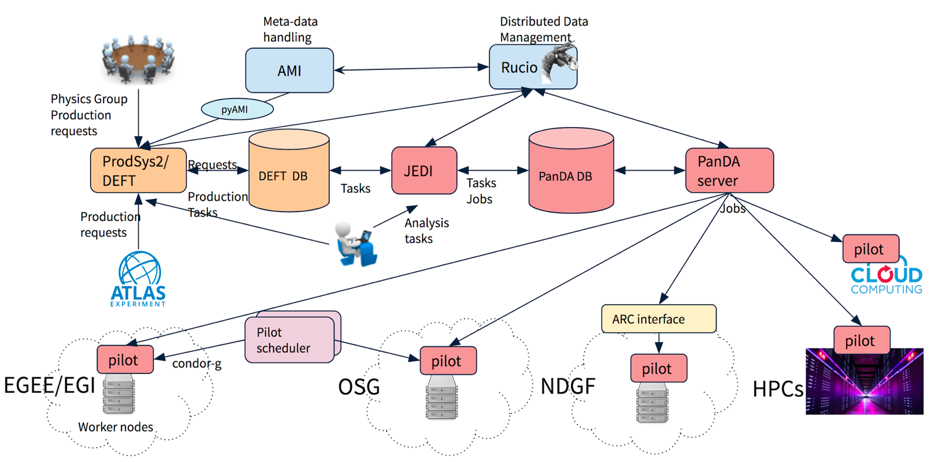
\includegraphics[width=0.90\textwidth]{figures/PanDA_architecture.png}
	\caption{PanDA architecture.}
	\label{fig:panda-arch}
\end{figure}

Since 2012 the BigPanDA project funded by Advanced Scientific Computing Research (ASCR) program ~\cite{DOEASCR} was aimed to extend PanDA beyond the Grid and High-Energy Physics (HEP). The project included many activities beyond ATLAS experiment and provided significant contribution to integration of the supercomputers including Titan~\cite{Titan} operating at the Oak Ridge Leadership Computing Facility (OLCF) into the ATLAS computing model. 

Since 2015 the BigPanDA project evolved into the  BigPanDA++ as the collaboration between Brookhaven National Laboratory (BNL), Oak Ridge National Laboratory (ORNL),  University of Texas Arlington (UTA) and Rutgers University.


% ---------------------------------------------------------------------------
\section{PanDA outside ATLAS and CERN: instances at OLCF and EC2 and user environment}

\subsection{PanDA Server instances in EC2 Amazon Cloud and OLCF}


ATLAS PanDA Server depends on Oracle database backend, which is a proprietary product. In order to meet licensing requirements, a version of PanDA Server has been developed to run with MySQL database, an open-source product published under GPLv2 license.  
We have ported database description to MySQL excluding ATLAS-specific stored procedures. PanDA Monitor has also been tested for operability with MySQL.

In order to run payloads for non-ATLAS experiments a dedicated instance of MySQL-based PanDA Server has been deployed in Amazon EC2.  
PanDA Monitor was also configured to display job information for this instance, as well as AutoPilot~\cite{PanDAPilotSubmission} which submits pilots into Grid environment. 
As of today, there are 36 computing element endpoints configured with this instance of AutoPilot. 
This instance also serves HPC resources at BNL, NERSC and Jefferson Lab (JLab) via Harvester~\ref{section_harvester} instances deployed on the front nodes of these resources. 
Currently this instance server payloads for such experiments and projects like LSST/DESC and LQCD mentioned in sections ~\ref{section_lsst_desc} and ~\ref{section_lqcd}.

Another  PanDA Server instance to serve experiments and projects at OLCF (Figure~\ref{fig:panda-OLCF}) was deployed as a container-based application in OpenShift cluster management system at OLCF. This approach can be reused for fast deployments in the future. Currently this instance serves experiments and projects like nEDM~\ref{section_nedm}, Computational Biology~\ref{section_biology}, IceCube~\ref{section_icecube} and Molecular Dynamics~\ref{section_moldyn}.
To isolate the workflows of different groups and experiments, the dedicated queues were defined for both PanDA Server instances. 
Presumably that on next steps we will provide the security mechanisms that will provide the grants to each queue only for dedicated users. 
Also, the PanDA provides the tools to customize environment variables, system settings and workflow algorithms for different user groups. 
Also, this split of the different groups workflows on the level of PanDA queues simplifies jobs monitoring via the web-based PanDA tool. 


\begin{figure}
  \centering
  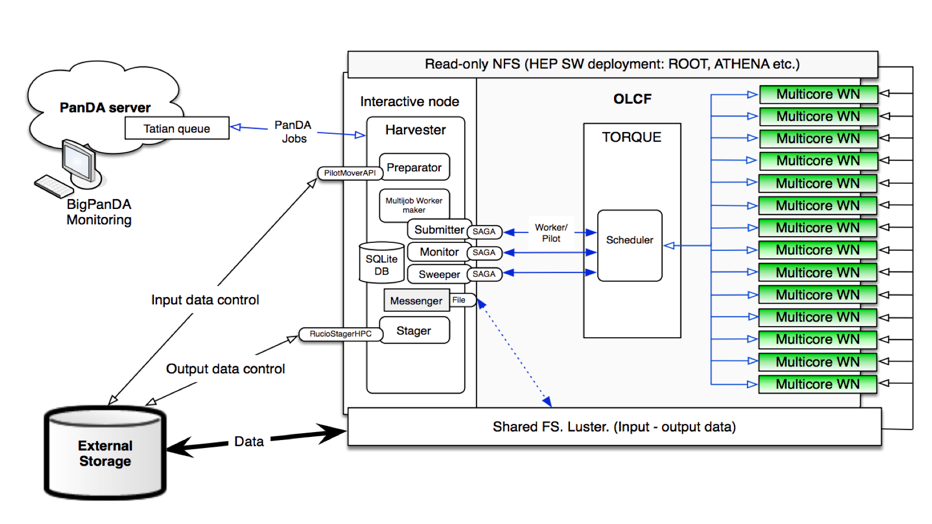
\includegraphics[width=0.90\textwidth]{figures/Panda_at_OLCF.png}
  \caption{Harvester architecture.}
  \label{fig:panda-OLCF}
\end{figure}

\subsection{From Pilot to Harvester} \label{section_harvester}

Pilot-based architecture~\cite{Nilsson_2008} allows PanDA to integrate the wide diversity of the computing architectures like Grid,  HPCs and Clouds. However, for correct operation pilot requires outbound network connection from worker nodes, which might be absent on worker nodes of HPCs, like Titan. In this case a persistent edge-service has to be used to submit jobs to local batch system.

Harvester~\cite{Megino_2017} is a resource-facing service between PanDA server and collection of workers on a compute site. It is intended to operate as a universal edge service in PanDA, capable of working with different types of computing resources -- Grid sites, clouds and supercomputers. Worker is a generalization of a pilot concept and can be, depending on a resource and workflow, a pilot, an MPI job, or a virtual machine. Harvester has modular multi-threaded design to support heterogeneous resources and to accommodate for special workflow requirements.

Harvester provides for flexible scheduling of job execution and asynchronous data transfer to and from the controlled resource.

We successfully used Harvester for integration of resources for various projects inside and outside of OLCF (Figure~\ref{panda-OLCF}). Harvester was used to run jobs on Titan for nEDM and LSST/DESC projects. It was used to integrate computational resources at BNL, JLab and NERSC for the Lattice QCD computations.

\subsection{Client tools: job description and description of workflows}

PanDa jobs are usually described using PanDA Framework entities. In order to provide an easier way to describe jobs a new job description format based on YAML has been introduced. This format includes necessary information to execute jobs on HPC resources: required walltime, payload script, etc. This new format also allows to describe simple workflows which can be executed by PanDA Server without any dependency on third-party services. This workflow description workflow supports description of independent jobs, jobs with multiple inputs and multiple outputs. In order to generate multiple similar parametrized workflows a template engine for workflow generation has also been introduced.

For easier job management a set of client tools has been developed. It allows the submission of jobs in YAML format, as well as job status polling and cancelation. A separate tool has been developed which allows to generate YAML job descriptions from templates. Workflow management tools are currently being developed.


% ---------------------------------------------------------------------------
%\section{RADICAL-Pilot and Next Generation Executor}\label{sec:rp}

\section{Experiments And Projects}
\subsection{PanDA for Computational Biology and Genomics} \label{section_biology}

In collaboration with Center for Bioenergy Innovation at ORNL, the PanDA based workflow for epistasis research~\cite{Gros277} was established.

% Epistasis is the phenomenon where the effect of one gene is dependent on the presence of one or more 'modifier genes', i.e. the genetic background. 

The GBOOST~\cite{GBOOST} application, a GPU-based tool for detecting gene-gene interactions in genome-wide case control studies, was used for initial tests. Input data were located in a set of eight input directories of 152 M each. Every PanDA job was configured to process single input directory in backfill mode on one node and walltime of 30 min. The output data of about 11M per job was located to the corresponding output directory.  

In 2019 we are going establish the workflow for larger scale computation runs on Titan and Summit~\cite{Summit}.

\subsection{PanDA for Molecular Dynamics} \label{section_moldyn}

In collaboration with department of Chemistry and Biochemistry at the University of Texas Arlington we implemented test to try out PanDA to support the Molecular Dynamics~\cite{3b6dad414e794d36954333f8f177f47c} study ''Simulating Enzyme Catalysis, Conformational Change, and Ligand Binding/Release''. 
The CHARMM (Chemistry at HARvard Macromolecular Mechanics) application was chosen as a basic payload tool. 
% CHARMM is a molecular simulation program with broad application to many-particle systems with a comprehensive set of energy functions, a variety of enhanced sampling methods, and support for multi-scale techniques including QM/MM, MM/CG, and a range of implicit solvent models. 
%CHARMM is a molecular simulation program which primarily targets biological systems including peptides, proteins, prosthetic groups, small molecule ligands, nucleic acids, lipids, and carbohydrates, as they occur in solution, crystals, and membrane environments, it is designed for hybrid MPI/OpenMP/GPU computing.
CHARMM is a molecular simulation program which primarily targets biological systems including peptides, proteins, prosthetic groups, and others; it is designed for hybrid MPI/OpenMP/GPU computing.
% CHARMM also finds broad applications for inorganic materials with applications in materials design. 
% CHARMM design for hybrid MPI/OpenMP/GPU computing. 
For initial tests with PanDA we configured two types of jobs with different run time and output data volumes. 
These tests were successfully run on Titan using job submission via PanDA server at OLCF .


\subsection{PanDA for IceCube} \label{section_icecube}

Together with experts from the IceCube~\cite{doi:10.1063/1.3480478} experiment we implemented the demonstrator for IceCube job submission to Titan using PanDA system . 
IceCube is a particle detector at the South Pole that records the interactions of a nearly massless subatomic particle called the neutrino. 
%Demonstrator includes the use of NuGen package (a modified version of ANIS~\cite{GAZIZOV2005203} that works with IceCube software) -- GPU application for atmospheric neutrinos are simulations packed in singularity container and remote stage-in/-out the data from GridFTP~\cite{GlobusGridFTP} storage with GSI authentication. 
%Demonstrator includes the use of NuGen package (a modified version of ANIS~\cite{GAZIZOV2005203} that works with IceCube software) -- GPU application for atmospheric neutrinos are simulations packed in singularity container and remote stage-in/-out the data from GridFTP~\cite{GridFTP_Proc} storage. 
Demonstrator includes the use of GPU simulation tools for atmospheric neutrinos, packed in Singularity container and remote stage-in/-out the data from a remote storage. 
Test jobs ran in one node mode with walltime of 120 minutes. After successful tests of this realistic IceCube jobs, we intended to perform full scale processing of 4500 files.


\subsection{PanDA for BlueBrain} \label{section_bluebrain}

In 2017, a pilot project was started between BigPanDA and the Blue Brain Project (BBP)~\cite{Markram:BBP} of the Ecole Polytechnique Federale de Lausanne (EPFL) located in Lausanne, Switzerland. This proof of concept project is aimed at demonstrating the efficient application of the PanDA system to support the complex scientific workflow of the BBP which relies on using a mix of desktop, cluster and supercomputers to reconstruct and simulate accurate models of brain tissue.

In the first phase of this joint project we supported the execution of BBP software on a variety of distributed computing systems powered by PanDA. 
%The targeted systems for demonstration included: Intel x86-NVIDIA GPU based BBP clusters located in Geneva (47 TFlops) and Lugano (81 TFlops), BBP IBM BlueGene/Q supercomputer (0.78 PFLops and 65 TB of DRAM memory) located in Lugano, the Titan Supercomputer with peak theoretical performance 27 PFlops operated by the Oak Ridge Leadership Computing Facility (OLCF), and Cloud based resources such as Amazon Cloud.
%The targeted systems for demonstration included: Intel x86-NVIDIA GPU based BBP clusters located in Geneva and Lugano, BBP IBM BlueGene/Q supercomputer located in Lugano, the Titan supercomputer at OLCF, and Cloud based resources such as Amazon Cloud.
The targeted systems for demonstration included: Intel x86-NVIDIA GPU based BBP clusters located in Geneva and Lugano, BBP IBM BlueGene/Q supercomputer in Lugano, the Titan supercomputer, and Cloud based resources such as Amazon Cloud.


In addition to standard PanDA components we developed the set of components to support BlueBrain user management, data flow, monitoring etc. 
Complete set of the tools provided within this project refers as PanDA portal and includes: Web-interface, Data Storage and Data Management System. 


\subsection{PanDa for LSST/DESC} \label{section_lsst_desc}

A goal of Large Synoptic Survey Telescope (LSST) project is to conduct a 10-year survey of the sky that is expected to deliver 200 petabytes of data after it begins full science operations in 2022. 
The project will address some of the most pressing questions about the structure and evolution of the universe and the objects in it. 
It will require a large amount of simulations, which model the atmosphere, optics and camera to understand the collected data. 
The LSST Dark Energy Science Collaboration (LSST/DESC)~\cite{lsst-desc} will prepare and perform a variety of cosmological analyses with the data received with LSST. 
This will allow provide the community with state of the art analysis tools which, in their turn, will help to expand the knowledge about dark energy.

For running LSST/DESC simulations with the PanDA WMS we have established a distributed testbed infrastructure that employs the resources of several sites on GridPP~\cite{GridPP_Collaboration_2005} and Open Science Grid~\cite{Pordes_2007} as well as the Titan supercomputer. In order to submit jobs to these sites we have used a PanDA server instance deployed on the Amazon AWS Cloud. 
Current LSST/PanDA computing environment includes 2 sites in Open Science Grid (US), 8 sites in GridPP (UK) and LAPP Grid Site (France). 
Currently there are 36 Grid endpoints that support LSST/DESC payloads. During our last tests we managed reach around 3000 simultaneously running LSST/DESC jobs via PanDA infrastructure without any dedicated resources. 
Job duration was 4-24 hours with average duration around 7.5 hours.
LSST/DESC workflows defined in YAML were tested with PanDA and Harvester as an edge service on NERSC Cori~\cite{NERSC_Cori}. ''2-point Statistics Analysis'' workflow (Figure~\ref{fig:lsst_desc_2pt_stats}) contains several steps where output from completed step is passed to the input of a next step. There were also intermediate steps that performed data preparation which had to be executed locally on a front node, main steps for the analysis were executed on worker nodes of Cori in Shifter containers prepared by BNL Astro group.



\begin{figure}
  \centering
  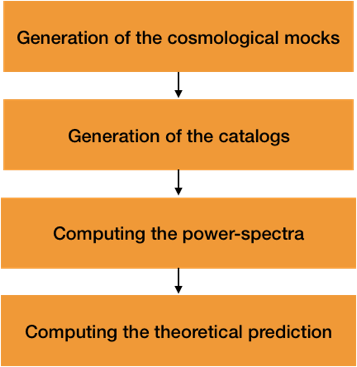
\includegraphics[width=0.30\textwidth]{figures/LSST_2point_statistics.png}
  \caption{2-point Statistics Analysis workflow}
  \label{fig:lsst_desc_2pt_stats}
\end{figure}


\subsection{PanDA for Lattice QCD computations} \label{section_lqcd}

%Lattice QCD (LQCD) is a well-established non-perturbative approach to solving the quantum chromodynamics theory of quarks and gluons.  
Quantum chromodynamics (QCD) is the fundamental theory to describe the dynamics of quarks and gluons in hadrons.
% Lattice QCD (LQCD) simulations~\cite{LQCD_Matsufuru} have become the most efficient tool to analyze the nonperturbative nature of QCD.
Lattice QCD (LQCD) simulations are the most efficient tools for nonperturbative analysis of QCD.
Current LQCD payloads can be characterized as massively parallel, occupying thousands of nodes on leadership-class supercomputers. 

The computations typically proceed in two phases: in the first phase, one generates thousands of configurations of the strong force fields (gluons), colloquially referred to as gauge fields. 
%This computation is a long-chain Monte Carlo process, requiring the focused power of leadership class computing facilities for extended periods. In the second phase, these configurations are analyzed on various HPC resources~\cite{Babich:2010:PQL:1884643.1884695}.
This computation is a long-chain Monte Carlo process, requiring the focused power of leadership class computing facilities for extended periods. In the second phase, these configurations are analyzed on various HPC resources~\cite{Babich:2011np}.
Until a few years ago, the analysis phase would often account for a relatively small part of the cost of the overall calculation. In recent years, however, focus has turned to more challenging physical observables and new analysis. As a result, the relative costs have shifted to the point where analysis often requires an equal or greater amount of computation than gauge field generation.

In 2017, as a part of SciDAC-4 funded project, a collaboration was formed between several US LQCD groups and BigPanDA team with the goal to adopt PanDA WMS for the needs of the SciDAC-4 LQCD computational program.

In order to run LQCD payloads we have used our PanDA Server in Amazon cloud. Production campaigns were executed on BNL Institutional Cluster through a dedicated instance of Harvester. During the period between April and June 2018 13 TB of input data were processed, producing output of 176 GB. LQCD jobs used around 15000 GPU hours with average job duration around 12 hours.

Another branch of LQCD activities is developed by Jefferson Lab. 
They have their own instance of Harvester deployed on the front node of JLab internal computing environment and an instance of Harvester on NERSC. The goal is to create a private computing segment which will consist of several JLab clusters and NERSC resources (Figure~\ref{fig:lqcd_env}).

Different LQCD groups are planning to share input data generated on Titan among other computing resources. We have successfully tested these data transfers performed by Harvester between OLCF and NERSC via Globus file sharing~\cite{Globusdatatransfer}.

In terms of preparation to future LQCD campaigns an instance of Harvester was successfully installed and tested on the front node of SummitDev supercomputer. It will be also available to other experiments and projects after Summit will be in full production.

\begin{figure}
	\centering
	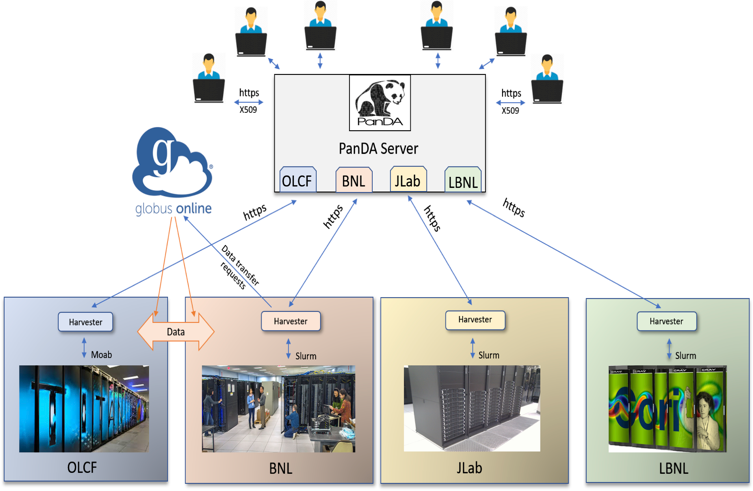
\includegraphics[width=0.60\textwidth]{figures/LQCD_future_environment.png}
	\caption{2-point Statistics Analysis workflow}
	\label{fig:lqcd_env}
\end{figure}


\subsection{PanDA for nEDM} \label{section_nedm}

Precision measurements of the properties of the neutron present an opportunity to search for violations of fundamental symmetries and to make critical tests of the validity of the Standard Model (SM) of electroweak (EW) interactions. 
% These experiments have been pursued with great energy and interest since the discovery of neutron in 1932.  
% The goal of the nEDM~\cite{Lamoreaux_2009} experiment at the Fundamental Neutron Physics Beamline at the Spallation Neutron Source (Oak Ridge National Laboratory) is to further improve the precision of this measurement by another factor of 100.
The goal of the nEDM~\cite{Lamoreaux_2009} experiment at ORNL is to further improve the precision of this measurement by another factor of 100.


Current nEDM payloads run detector simulations using GEANT4~\cite{AGOSTINELLI2003250} with walltime around 20 minutes. We have successfully tested nEDM payloads executed through Harvester instance deployed on a login node of Titan supercomputer. No specific data movement was required from nEDM; input and output data remain on Titan’s Lustre filesystem. nEDM team is planning to run their data challenges in 2019 through OLCF PanDA Server instance.


% ---------------------------------------------------------------------------
\section{Conclusions}

In terms of BigPanDA project we are making research on how PanDA features can be useful not only for ATLAS, but to non-ATLAS and non-HEP experiments and projects.
The most remarkable achievements for now for BigPanDA project beyond ATLAS are the following:

\begin{itemize}
	\item we created a version of PanDA Server, which does not 	depend on proprietary software
	\item several PanDA Server instances were deployed to serve different non-ATLAS payloads
	\item application from several projects (LSST/DESC, nEDM, BlueBrain, Molecular Dynamics, Computational Biology, LQCD) were executed via PanDA on various Grid and HPC resources
	\item production campaign has been started for LQCD computations on BNL Institutional Cluster
	\item automated data transfer instruments have been tested with PanDA for non-ATLAS experiment on heterogeneous resources
\end{itemize}

The future goals for BigPanDA regarding non-ATLAS projects and experiments are:

\begin{itemize}
	\item to integrate new Grid and HPC resources that will be served with PanDA Servers
	\item to prepare for payloads and workflows that will be run on next-generation HPCs like Summit
\end{itemize}

\bigskip

%\section{Acknowledgements}

%This work was funded in part by the U.S. Department of Energy, Office of Science, High Energy Physics and Advanced Scientific Computing Research under Contracts DE-SC0008635, DE-SC0016280. We would like to acknowledge that this research used resources of the Oak Ridge Leadership Computing Facility at the Oak Ridge National Laboratory, which is supported by the Office of Science of the U.S. Department of Energy under Contract no. DE-AC05-00OR22725.

\begin{acknowledgement}
	This work was funded in part by the U.S. Department of Energy, Office of Science, High Energy Physics and Advanced Scientific Computing Research under Contracts DE-SC0008635, DE-SC0016280. We would like to acknowledge that this research used resources of the Oak Ridge Leadership Computing Facility at the Oak Ridge National Laboratory, which is supported by the Office of Science of the U.S. Department of Energy under Contract no. DE-AC05-00OR22725.
\end{acknowledgement}


% ---------------------------------------------------------------------------
% Bibliography
% ---------------------------------------------------------------------------
%\bibliography{main}
\bibliography{panda}

\end{document}
